\documentclass[
	% -- opções da classe memoir --
	12pt,				% tamanho da fonte
	%openright,			% capítulos começam em pág ímpar (insere página vazia caso preciso)
	oneside,			% p/ impressão frente e verso:
	%					%oneside -> Normal. 
	%					%twoside -> insere página antes e depois de cada capítulo
	a4paper,			% tamanho do papel. 
	% -- opções da classe abntex2 --
	%chapter=TITLE,		% títulos de capítulos convertidos em letras maiúsculas
	%section=TITLE,		% títulos de seções convertidos em letras maiúsculas
	%subsection=TITLE,	% títulos de subseções convertidos em letras maiúsculas
	%subsubsection=TITLE,% títulos de subsubseções convertidos em letras maiúsculas
	% -- opções do pacote babel --
	english,			% idioma adicional para hifenização
	french,				% idioma adicional para hifenização
	spanish,			% idioma adicional para hifenização
	brazil				% o último idioma é o principal do documento
	]{abntex2}
% ---
% Pacotes básicos 
% ---
\usepackage{lmodern}			% Usa a fonte Latin Modern			
\usepackage[T1]{fontenc}		% Selecao de codigos de fonte.
\usepackage[utf8]{inputenc}		% Codificacao do documento (conversão automática dos acentos)
\usepackage{indentfirst}		% Indenta o primeiro parágrafo de cada seção.
\usepackage{color}				% Controle das cores
\usepackage{graphicx}			% Inclusão de gráficos
\usepackage{microtype} 			% para melhorias de justificação

% ---
% Atribuições Matemáticas 
% ---
\usepackage{amsmath, amsfonts, amssymb} % pacotes para caracteres extras
\DeclareMathOperator{\sen}{sen}
\DeclareMathOperator{\arcsen}{arcsen}
\DeclareMathOperator{\tg}{tg}
\DeclareMathOperator{\cossec}{cossec}
\newcommand{\limite}{\displaystyle\lim}
\newcommand{\integral}{\displaystyle\int}
		
% ---
% Pacotes de citações
% ---
\usepackage[brazilian,hyperpageref]{backref}	 % Paginas com as citações na bibl
\usepackage[alf]{abntex2cite}	% Citações padrão ABNT

% --- 
% CONFIGURAÇÕES DE PACOTES
% --- 

% ---
% Configurações do pacote backref
% Usado sem a opção hyperpageref de backref
\renewcommand{\backrefpagesname}{Citado na(s) página(s):~}
% Texto padrão antes do número das páginas
\renewcommand{\backref}{}
% Define os textos da citação
\renewcommand*{\backrefalt}[4]{
	\ifcase #1 %
		Nenhuma citação no texto.%
	\or
		Citado na página #2.%
	\else
		Citado #1 vezes nas páginas #2.%
	\fi}%
% ---

% ---
% Informações de dados para CAPA e FOLHA DE ROSTO
% ---
\titulo{TÍTULO: \\ \textbf{Subtítulo}}
\autor{Nome do Autor}
\local{Local, AA - Brasil}
\data{\today}
%\orientador{Professor}

\tipotrabalho{Relatório Experimental}
% O preambulo deve conter o tipo do trabalho, o objetivo, 
% o nome da instituição e a área de concentração 
\preambulo{Relatório referente à terceira experiência de óptica realizada no dia 21 de setembro de 2017,para obtenção parcial da segunda nota da disciplina Física Experimental II. \newline \newline Prof. Nome do Professor.}
% ---


% ---
% Configurações de aparência do PDF final

% alterando o aspecto da cor azul
\definecolor{blue}{RGB}{41,5,195}

% informações do PDF
\makeatletter
\hypersetup{
     	%pagebackref=true,
		pdftitle={\@title}, 
		pdfauthor={\@author},
    	pdfsubject={\imprimirpreambulo},
	    pdfcreator={LaTeX with abnTeX2},
		pdfkeywords={abnt}{latex}{abntex}{abntex2}{trabalho acadêmico}, 
		colorlinks=true,       		% false: boxed links; true: colored links
    	linkcolor=blue,          	% color of internal links
    	citecolor=blue,        		% color of links to bibliography
    	filecolor=magenta,      		% color of file links
		urlcolor=blue,
		bookmarksdepth=4
}
\makeatother
% --- 

% --- 
% Espaçamentos entre linhas e parágrafos 
% --- 

% O tamanho do parágrafo é dado por:
\setlength{\parindent}{1.3cm}

% Controle do espaçamento entre um parágrafo e outro:
\setlength{\parskip}{0.2cm}  % tente também \onelineskip

% ---
% compila o indice
% ---
\makeindex
% ---

% ----
% Início do documento
% ----
\begin{document}

% Seleciona o idioma do documento (conforme pacotes do babel)
%\selectlanguage{english}
\selectlanguage{brazil}

% Retira espaço extra obsoleto entre as frases.
\frenchspacing 

% ----------------------------------------------------------
% ELEMENTOS PRÉ-TEXTUAIS
% ----------------------------------------------------------
\pretextual

\begin{center}			
	\begin{figure}[htb]
		\centering
		
\includegraphics[scale=0.15]{ufmalogo.jpg}
	\end{figure}
				
			\textbf{UNIVERSIDADE FEDERAL DO MARANHÃO \\
					CENTRO DE CIÊNCIAS EXATAS E TECNOLOGIAS \\
					DEPARTAMENTO \\
					CURSO\\\vspace{5cm}}
					
					\textbf{\large{TÍTULO:}\\
					\large{Subtítulo}}
					\vspace{3.5cm}
					\begin{flushright}
						\textnormal{Nome do Autor}
					\end{flushright}
					\vspace{4.5cm}
					\textbf{São Luís, MA \\ \today}
\end{center}

% ---
% Folha de rosto
% (o * indica que haverá a ficha bibliográfica)
% ---
\imprimirfolhaderosto
% ---
% ---
% RESUMOS
% ---

% resumo em português
\setlength{\absparsep}{18pt} % ajusta o espaçamento dos parágrafos do resumo
\begin{resumo}
Este relatório é referente ao experimento de física II, a abordar os conceitos sobre desvio lateral da luz. Fenômeno que ocorre em uma lâmina de faces paralelas, sistema constituído de três meios homogêneos e transparentes separados dois a dois através de superfícies planas e paralelas, o que permite fazer com que um raio monocromático de luz seja desviado sem alterar sua direção de propagação, ocorrendo apenas um desvio lateral. Neste experimento, observou-se os raios refratados a fim de obter experimentalmente o índice de refração absoluto da lâmina e o valor do desvio lateral da luz sofrido, fundamentado na Lei de Snell Descartes.\\
\thispagestyle{plain}
\textbf{Palavras chave:}  desvio lateral da luz; lâmina de faces paralelas; Lei de Snell-Descartes.
\end{resumo}


% ---
% inserir o sumario
% ---
\pdfbookmark[0]{\contentsname}{toc}
\tableofcontents*
\cleardoublepage
% ---

% ----------------------------------------------------------
% ELEMENTOS TEXTUAIS
% ----------------------------------------------------------
\textual

% ----------------------------------------------------------
% Introdução (exemplo de capítulo sem numeração, mas presente no Sumário)
% ----------------------------------------------------------
\chapter{Introdução}
% ----------------------------------------------------------

Há inúmeros dispositivos ópticos constituídos de corpos transparentes limitados por duas superfícies, planas ou curvas. Essas superfícies são dioptros, pois separam esses corpos dos meios que estão imersos (quase sempre o ar) e modificam a trajetória dos raios de luz que os atravessam, alterando a posição ou modificando as dimensões das coisas que vemos através deles. Se essas superfícies forem planas, a forma do objeto observado não se altera, sofrendo apenas uma mudança de posição. É o caso das lâminas de faces paralelas \cite{gaspar}.

O desvio lateral da luz é um fenômeno físico que ocorre quando um feixe de luz, ao passar para um meio com índice de refração diferente, sofre um desvio angular com relação a normal causado pelo fenômeno da refração no qual devido à mudança da velocidade do feixe de luz ao viajar entre meios ópticos diferentes muda a angulação de sua trajetória \cite{merefrac}.

No século XVII, o matemático e astrônomo holandês Willebrord Snellius \cite{wikiroyen}, ficou conhecido por elaborar uma expressão que era possível prever o desvio angular sofrido pela luz ao passar de um meio para outro com índices de refração diferentes. Essa expressão ficou conhecia como lei de Snell (ou Lei de Snell-Descartes), que consiste na igualdade do produto do índice de refração pelo seno do ângulo de incidência do meio um, pelo produto do índice de refração pelo seno do ângulo de refração do meio dois \cite{wikisneel}.

O fenômeno é estudado observando um feixe de luz passando por laminas de faces paralelas, no qual, ao passar do ar (meio um) para o vidro (meio dois) sofre um desvio lateral que posteriormente é corrigido ao passar pela outra lâmina de vidro para o ar.

\chapter{Abordagem Teórica}

\textbf{Desvio Lateral da Luz}

Seja $L$ uma lâmina transparente de faces paralelas e planas, constituindo um conjunto de três meios homogêneos e transparentes. Pode-se considerar este modelo como um sistema resultante da associação de dioptros planos. Dioptro é definido por um sistema constituído por meios homogêneos e transparentes.
Para configuração da lâmina de faces paralelas, pode-se observar o aparecimento de duas refrações, visto que uma ocorre quando a luz incide sobre a primeira face plana adentrando o material e a outra, quando a luz incide sobre a segunda face, saindo. Portanto, a lâmina de faces paralelas e planas é um dispositivo que propicia um desvio na direção de propagação da luz em um determinado meio \cite{resnick4}.

\begin{figure}[htb]
	\centering
	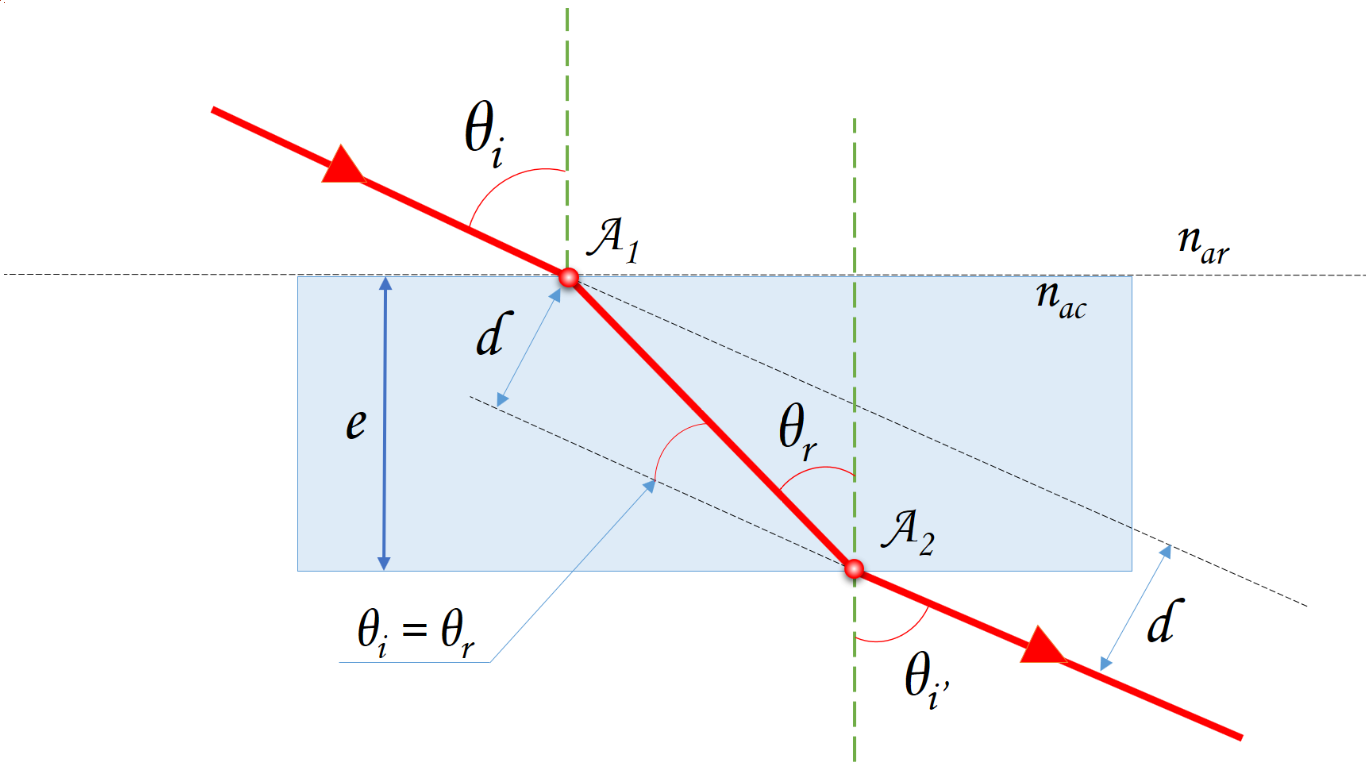
\includegraphics[scale=0.3]{Imagem1.png}
	\caption{Representação do Desvio Lateral da Luz.}
	\label{figura-1}
\end{figure}

Sendo o ângulo de incidência $\theta_i$, então a relação entre os ângulos de incidência e refretado, $\theta_r$, é regida pela Lei de Snell-Descartes, logo, tem-se como resultado para a primeira refração:

$$n_{ar} \cdot sen(\theta_i) = n_{ac} \cdot sen(\theta_r)$$

Muitos materiais possuem seu índice de refração conhecido, a tabela seguinte mostra alguns deles:

\begin{table}[htb]
	\centering
	\begin{tabular}{c|c}
		\hline		
		Meio Material & Índice de Refração($n$) \\
		\hline
		Ar & $1,00$ \\
		Água & $1,33$ \\
		Vidro & $1,50$ \\
		Acrílico & $1,49$ \\
		Diamante & $2,42$ \\
		\hline
	\end{tabular}
	\caption{Índice de Refração($n$) de alguns meios materiais - \cite{usprefrac}}
	\label{tabela-índice_n}
\end{table}

\newpage

Na segunda refração, o ângulo de incidência é $\theta_r$, que incide sobre a face interna da lente e refrata para fora do material, $\theta_{i'}$. Utilizando-se, novamente, da Lei de Snell-Descartes, obtém-se:

$$n_{ac} \cdot sen(\theta_r) = n_{ar} \cdot sen(\theta_{i'})$$

Assim, pode-se descrever $\theta_i$ = $\theta_{i'}$.

Portanto, é recorrente a verificação que em tal configuração de lâmina não há variação angular. Todavia, a ocorrência do deslocamento linear é eminente, logo, existe um notável desvio lateral da luz.

$$sen(\theta_i - \theta_r) = \dfrac{d}{A_1A_2}$$

$$cos(\theta_r) = \dfrac{A_1B}{A_1A_2}$$

Onde $A_1B$ equivale a espessura da lâmina, denominada por $e$. Utilizando-se das equações do seno e cosseno acima, tem-se:

$$\dfrac{A_1}{cos(\theta_r)} = \dfrac{d}{sen(\theta_i - \theta_r)}$$

$$d = \dfrac{A_1B \cdot sen(\theta_i - \theta_r)}{cos(\theta_r)}$$

Substituindo $A_1B$ por e, fica-se com:

$$d = e \cdot \dfrac{sen(\theta_i - \theta_r)}{cos(\theta_r)}$$


\chapter{Procedimentos Experimentais}
\section{Materiais}

Para montagem do referido experimento, utilizou-se os seguintes materiais:

$1$ - Lâmina de Acrílico;

$2$ - Fonte de luz;

$3$ - Paquímetro;

$4$ - Banco Óptico; 

$5$ - Régua; 


\begin{figure}[htb]
	\centering
	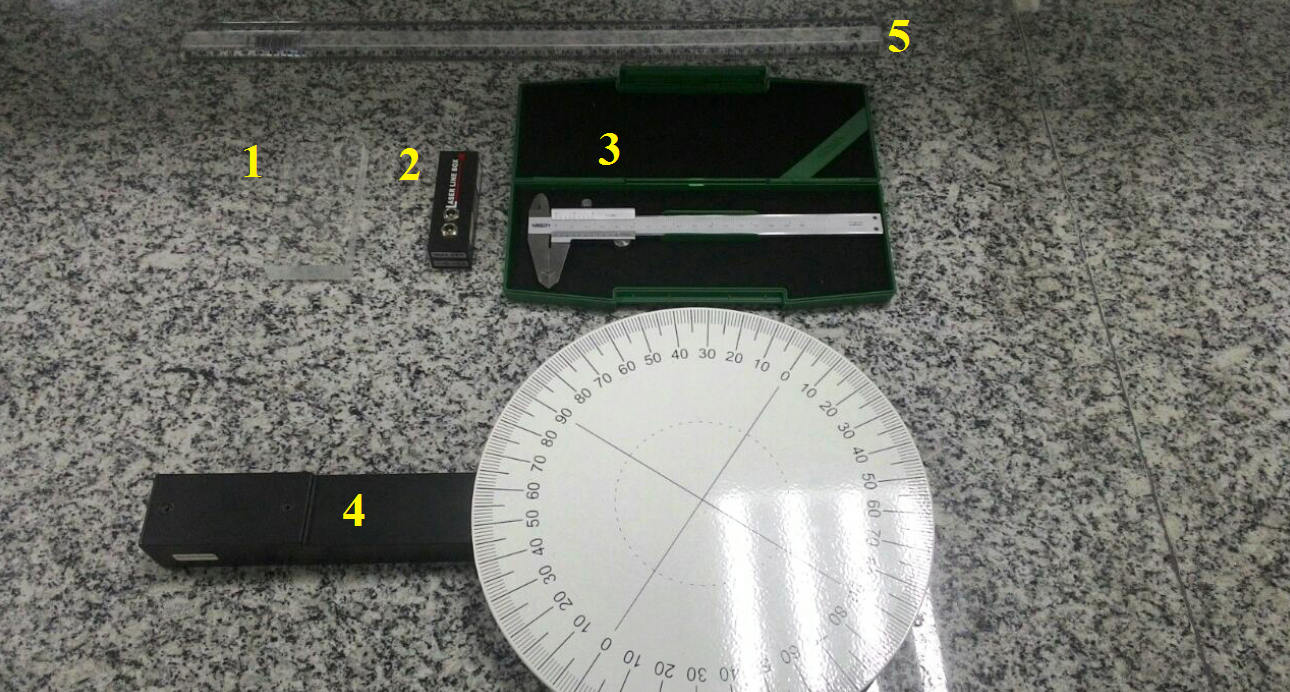
\includegraphics[scale=0.3]{materiais.png}
	\caption{Materiais Utilizados}
	\label{figura-materiais}
\end{figure}

\section{Métodos}

Inicialmente montou-se o equipamento, mediu-se a espessura da lâmina de faces paralelas através do paquímetro e posicionou-se a fonte de luz e a lâmina sobre disco graduado. Em seguida, ligou-se a fonte para emitir o feixe de luz incidente sobre a lâmina, ajustou-se o disco para o ângulo de $10\,^{\circ}$ e verificou-se que a luz sofreu um desvio lateral no segundo meio do corpo. Então, utilizou-se a régua para estender esse feixe de luz desviado no disco e conhecer o ângulo correspondente. Após isso, utilizou-se o paquímetro para medir a distância entre o ângulo da luz desviada e o ângulo de refração. O mesmo procedimento foi realizado para os ângulos de $20\,^{\circ}$, $30\,^{\circ}$, $40\,^{\circ}$, $50\,^{\circ}$, $60\,^{\circ}$ e $70\,^{\circ}$.


\chapter{Resultados}
%=================================================================================================================================================
%=================================================================================================================================================
\begin{flushleft}
\textbf{Obtenção do índice de refração absoluto da lâmina e os erros}
\end{flushleft}

Sabendo que $n_{Ar}\sen(\theta_i) = n_{ac}\sen(\theta_r)$ e que $n_{ac}(\theta_i , \theta_r)$, temos:

\begin{flushleft}
$ n_{ac} = \dfrac{n_{Ar} \cdot \sen(\theta_i)}{\sen(\theta_r)}$ onde $n_{Ar} = 1$, logo:

 $ n_{ac} = \dfrac{\sen(\theta_i)}{\sen(\theta_r)}$

$ n_{ac} = \overline{n}_{ac} \pm \Delta n_{ac}$

$ \Delta n_{ac} = \left|\dfrac{\partial n_{ac}}{\partial \theta_i}\right| \cdot \Delta \theta_i + \left|\dfrac{\partial n_{ac}}{\partial \theta_r}\right| \cdot \Delta \theta_r$

Derivando $ n_{ac}$ em função de $\theta_i$ e $\theta_r)$ temos:

$\left|\dfrac{\partial n_{ac}}{\partial \theta_i}\right| = \dfrac{\partial}{\partial \theta_i} \left(\dfrac{\sen(\theta_i)}{\sen(\theta_r)}\right) = \cos(\theta_i)cossec(\theta_r)$

$\left|\dfrac{\partial n_{ac}}{\partial \theta_r}\right| = \dfrac{\partial}{\partial \theta_r} \left(\dfrac{\sen(\theta_i)}{\sen(\theta_r)}\right) = sen(\theta_i) \cdot \cot(\theta_r) \cdot \cossec(\theta_r)$

logo,

$\Delta n_{ac} = \{\cos(\theta_i)cossec(\theta_r)\} \cdot \Delta \theta_i + \{\sen(\theta_i) \cdot \cot(\theta_r) \cdot \cossec(\theta_r)\} \cdot \Delta \theta_r$

Simplificando a equação encontrada, sabendo que $\Delta \theta_i = \Delta \theta_r$ temos que:

$\Delta n_{ac} = \Delta \theta_i \lbrack cossec^2(\theta_i) \cdot sen(\theta_i + \theta_r) \rbrack$

\end{flushleft}

Obtivemos que a média dos ângulo de incidência $(\theta_i) = 40 \,^{\circ} = 0,70  \;  rad$ e a média dos ângulos de refração $(\theta_r) = 24,3 \,^{\circ} = 0,42 \; rad$, onde $\Delta \theta_i = \Delta \theta_r = 0,5 \,^{\circ} \;  rad$ e  como $n_{ac}$ deve ser admensional então devemos transformar todos os ângulos em graus para radianos. Convertendo os ângulos para radianos e substituindo esses valores na equação obtida temos:

$\Delta n_{ac} = 0,01 \cdot \lbrack(cossec^2(0,7) \cdot sen(0,7 + 0,42)\rbrack$

$\Delta n_{ac} = 0,05$

Aplicamos este cálculo para todos os ângulos, obtendo assim uma média dos índices de refração e o desvio padrão que pode ser observado na tabela \ref{tabela-2} na página \pageref{tabela-2}. Então temos que o valor mais provável do índice de refração absoluto é:

\begin{table}[!htb]
	\centering
	\begin{tabular}{|c|}
		\hline
		$ n_{ac} = (1,49 \pm 0,05)$\\
		\hline
	\end{tabular}
\end{table}
\newpage

%=====================================================================================================================================================
%=====================================================================================================================================================
\begin{flushleft}
\textbf{Obtenção do desvio lateral da luz e os erros}
\end{flushleft}

Obtivemos que a média dos ângulo de incidência $(\theta_i) = 40 \,^{\circ} = 0,70 \; rad$ e a média dos ângulos de refração $(\theta_r) = 24,3 \,^{\circ} = 0,42 \; rad$ e $e=0,0501 m $. Sabemos também que a  equação do desvio lateral da luz é expressada por:

$$d = e \cdot \dfrac{sen(\theta_i - \theta_r)}{\cos(\theta_r)}$$

Convertendo todos os ângulos para radianos e substituindo esses valores na equação do desvio lateral da luz, temos:

$d = 0,0501 \cdot \dfrac{sen(0,70 - 0,42)}{\cos(0,42)} = 0,015 \; m$

Porém sabemos que $d(e, \theta_i, \theta_r)$, então devemos calcular os erros:

\begin{flushleft}
$ d = \overline{d} \pm \Delta d$

$ \Delta d = \left|\dfrac{\partial d}{\partial e}\right| \cdot \Delta e + \left|\dfrac{\partial d}{\partial \theta_i}\right| \cdot \Delta \theta_i + \left|\dfrac{\partial d}{\partial \theta_r}\right| \cdot \Delta \theta_r$

Derivando $d$ em função de $e, \theta_i$ e $\theta_r$, temos:

$\left|\dfrac{\partial d}{\partial e}\right| = \dfrac{\partial}{\partial e} \left(e \cdot \dfrac{sen(\theta_i - \theta_r)}{\cos(\theta_r)}\right) = \sec(\theta_r) \sen(\theta_i - \theta_r)$

$\left|\dfrac{\partial d}{\partial \theta_i}\right| = \dfrac{\partial}{\partial \theta_i} \left(e \cdot \dfrac{sen(\theta_i - \theta_r)}{\cos(\theta_r)}\right) = e\sec(\theta_r) \cos(\theta_i - \theta_r)$

$\left|\dfrac{\partial d}{\partial \theta_r}\right| = \dfrac{\partial}{\partial \theta_r} \left(e \cdot \dfrac{sen(\theta_i - \theta_r)}{\cos(\theta_r)}\right) = e\cos(\theta_i) \sec^2(\theta_r)$ \; logo,

$\Delta d = \lbrack \sec(\theta_r) \sen(\theta_i - \theta_r) \rbrack \cdot \Delta e + \lbrack e\sec(\theta_r) \cos(\theta_i - \theta_r)\rbrack \cdot \Delta \theta_i + \lbrack e\cos(\theta_i) \sec^2(\theta_r)\rbrack \cdot \Delta \theta_r$
\end{flushleft}

Obtivemos que a média dos ângulo de incidência $(\theta_i) = 40 \,^{\circ} = 0,70 \; rad$ e a média dos ângulos de refração $(\theta_r) = 24,3 \,^{\circ} = 0,42 \; rad$, onde $\Delta \theta_i = \Delta \theta_r = 0,5 \,^{\circ} = 0,01 \; rad$, $e=0,0501 m $ e $\Delta e = 5,00 \times 10^{-5}$. Convertendo todos os ângulos para radianos e substituindo esses valores na equação obtida temos:

$\Delta d = \lbrack \sec(0,42) \sen(0,70 - 0,42) \rbrack \cdot 5,00 \times 10^{-5} + \lbrack 0,0501 \sec(0,42) \cos(0,70 - 0,42)\rbrack \cdot 0,01 + \lbrack 0,0501 \cos(0,70) \sec^2(0,42)\rbrack \cdot 0,01$

$$\Delta d = 0,009 m$$

Aplicamos este cálculo para todos os ângulos, obtendo assim uma média dos índices de refração e o desvio padrão que pode ser observado na tabela \ref{tabela-2} na página \pageref{tabela-2}. Então temos que o valor mais provável do desvio lateral da luz é:

\begin{table}[!htb]
	\centering
	\begin{tabular}{|c|}
		\hline
		$d = (0,015 \pm 0,009) m$\\
		\hline
	\end{tabular}
\end{table}


\newpage
%=====================================================================================================================================================
%=====================================================================================================================================================
A seguinte tabela mostra os ângulos de refração($\theta_r$), os índices de refração e os desvios laterais que foram obtidos a partir dos ângulos de incidência($\theta_i$), onde a luz atingiu o ar e depois o acrílico: 

\begin{table}[htb]
	\centering
	\begin{tabular}{c|c|c|c}
		\hline		
		($\theta_i$) & ($\theta_r$) & Índ. de Refração($n_{ac}$) & Desvio Lateral ($d$)\\
		\hline
		$(10\pm 0,5)\,^{\circ}$ & $(7 \pm 0,5)\,^{\circ}$ & $(1,42 \pm 0,009)$ & $(0,002 \pm 0,0013)m$\\
		$(20\pm 0,5)\,^{\circ}$ & $(13 \pm 0,5)\,^{\circ}$ & $(1,52 \pm 0,006)$ & $(0,006 \pm 0,0009)m$\\
		$(30\pm 0,5)\,^{\circ}$ & $(19 \pm 0,5)\,^{\circ}$ & $(1,54 \pm 0,007)$ & $(0,009 \pm 0,0007)m$\\
		$(40\pm 0,5)\,^{\circ}$ & $(25 \pm 0,5)\,^{\circ}$ & $(1,52 \pm 0,014)$ & $(0,013 \pm 0,0006)m$\\
		$(50\pm 0,5)\,^{\circ}$ & $(31 \pm 0,5)\,^{\circ}$ & $(1,49 \pm 0,125)$ & $(0,019 \pm 0,0005)m$\\
		$(60\pm 0,5)\,^{\circ}$ & $(35 \pm 0,5)\,^{\circ}$ & $(1,51 \pm 0,094)$ & $(0,024 \pm 0,0004)m$\\
		$(70\pm 0,5)\,^{\circ}$ & $(40 \pm 0,5)\,^{\circ}$ & $(1,46 \pm 0,014)$ & $(0,032 \pm 0,0006)m$\\		
		\hline
		\multicolumn{2}{c|}{Média} &$1,49$ & $0,015 m$\\
		\hline
		\multicolumn{2}{c|}{Desvio Padrão} &$0,05$ & $0,009 m$\\
		\hline
		\multicolumn{2}{c|}{Valor mais Provável} &$(1,49 \pm 0,05)$ &  $(0,015 \pm 0,009)m$\\
		\hline		
	\end{tabular}
	\caption{Tabela dos dados obtidos}
	\label{tabela-2}
\end{table}

%=================================================================================================================================================
O gráfico com barra de erros a seguir mostra o comportamento do ângulo de incidência($\theta_i$) em função do ângulo de refração($\theta_r$):

\begin{figure}[htb]
	\centering
	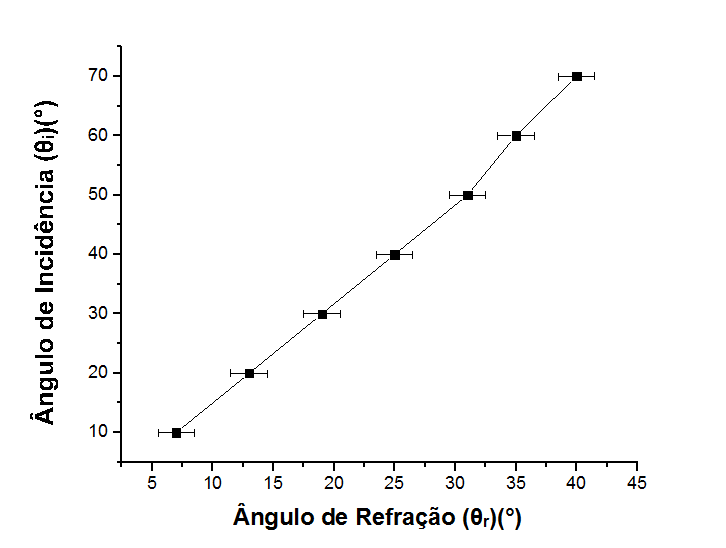
\includegraphics[scale=0.7]{Grafico1.png} 
	\caption{Ângulo de incidência($\theta_i$) em função do ângulo de refração($\theta_r$)}
	\label{figura-grafico2}
\end{figure}
\newpage

A figura a seguir mostra que foi possível observar o fenômeno de desvio lateral da luz:

\begin{figure}[htb]
	\centering
	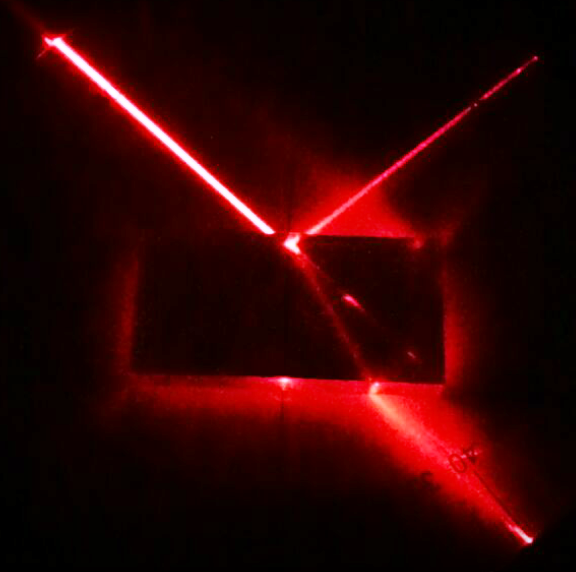
\includegraphics[scale=0.8]{desvio.png}
	\caption{Imagem obtida no momento do experimento}
	\label{figura-8}
\end{figure}

\newpage
%=====================================================================================================================================================
%=====================================================================================================================================================

% ----------------------------------------------------------
% Finaliza a parte no bookmark do PDF
% para que se inicie o bookmark na raiz
% e adiciona espaço de parte no Sumário
% ----------------------------------------------------------
\phantompart


\chapter{Conclusão}
De acordo com as fórmulas e todo o material disponível sobre o assunto, foi possível realizar os devidos cálculos e comprovar matematicamente o desvio lateral da luz observado no laboratório. A distância($d = (0,015 \pm 0,009)m$) a qual mede o desvio lateral sofrido pelo raio de luz, foi encontrada por intermédio dos cálculos que se mostrou favorável, pois os resultados obtidos foram próximos e dentro da margem de erro ao que foi medido com o paquímetro($d = 0,020m$), assim como o índice de refração da lâmina ($n_{ac} = 1,49 \pm 0,05$)) conforme o índice de refração do acrílico mostrado na tabela \ref{tabela-índice_n}, na página \pageref{tabela-índice_n}. Assim pode-se afirmar que o experimento foi conduzido de forma eficaz. No experimento os raios de luz de incidência e o de emergência mostraram-se paralelos, de acordo com a literatura isso mostra que o primeiro meio e terceiro meio são iguais, logo puderam-se realizar as relações trigonométricas e a lei de Snell-Descartes, para se processar os dados e encontrar os devidos resultados.

% ----------------------------------------------------------
% ELEMENTOS PÓS-TEXTUAIS
% ----------------------------------------------------------
\postextual
% ----------------------------------------------------------

% ----------------------------------------------------------
% Referências bibliográficas
% ----------------------------------------------------------
%\bibliography{abntex2-modelo-references}
\bibliography{referencia}

\end{document}
